\section{Description générale}

Sur demande de Jérôme DELATOUR pour le groupe ESEO, l'idée est de développer, à long terme, en collaboration avec un acteur industriel, un robot nettoyeur (aspiration + lavage) pour des structures industrielles.

Ce robot devra pouvoir nettoyer de grandes surfaces durant la nuit, surface répartie sur plusieurs niveaux. Le robot devra pouvoir donc prendre des monte-charges pour changer de niveaux. Il devra pouvoir aussi accéder à des bases de rechargement réparties dans tout le bâtiment (gestion énergie, mais aussi consommables pour le nettoyage, eau sale/propre, sac à vider, produit d'entretien).

Ici donc allons donc développer la partie logicielle de la Télécommande en Android Java et du Robot nettoyeur en C. Il sera question de développer un algorithme de déplacement et de gestion de ce robot avec aussi l'application Android qui servira de télécommande pour gérer au besoin le robot.

\subsection{Caractéristique des acteurs}

Par le terme d'acteur, nous désignons tout rôle joué par une entité (morale ou physique) qui interagit directement ou non avec le SàE. Cette entité peut être une personne (généralement un utilisateur du système) ou un autre système. Nous distinguons les acteurs, dits directs (qui interagissent directement avec le SàE) et les acteurs dits indirects (qui n'ont pas d'interaction directe avec le SàE) mais qui sont à l'origine d'exigences à respecter par le SàE.

\subsubsection{Acteurs directs}

\begin{itemize}
    \item \textbf{ROBOT} : Dans l'incrément 1 représente le logiciel de simulation et dans le 2 le robot piloté.
    \item \textbf{USER} : L'acteur qui interagit avec le simulateur/robot à travers l'application mobile développée. Cet acteur peut piloter le simulateur et observer l'état de fonctionnement du système et les alarmes de celui-ci.
\end{itemize}

\subsubsection{Acteurs indirects}

\begin{itemize}
    \item \textbf{Fournisseur électrique} : Source d'énergie pour alimenter le robot dans l'incrément 2
    \item \textbf{Normes}
\end{itemize}

\subsection{Environnement de développement}

Dans ce chapitre, il sera défini la frontière entre le Système à l'étude (SàE) et les entités qui l'environnent et interagisse avec lui.

\subsubsection{Architectures matérielle et logicielle}

Le SàE est constituer dans un premier temps d'un soft embarqué sur un PC hébergent le Simulateur du robot, ce soft étant l'algorithme de déplacement fait appelle à une bibliothèque fournie par le Client pour les fonctions de commande et de communication avec le robot. Cet ensemble peut communiquer avec une télécommande de type smartphone sur le quelle le soft Android est hébergée servant à pouvoir prendre le contrôle du robot et aussi récupérer les métriques de ce dernier.

\begin{figure}[H]
    \center
    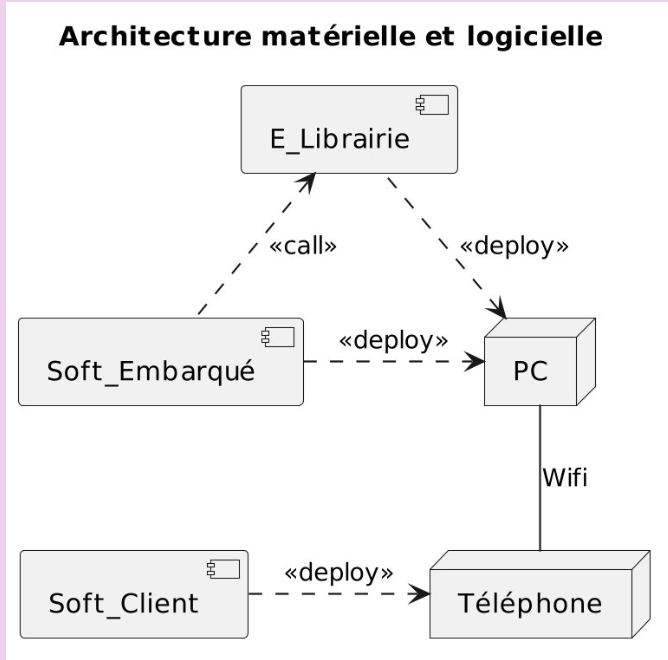
\includegraphics[scale=0.25]{data/arch_mat_log.png}
    \caption{Architecture matérielle et logicielle}
    \label{fig:architecture}
\end{figure}

Le testeur doit pouvoir communiquer avec le SAE via une application Android.

\subsubsection{Contexte logique}

Cette partie décrit les entrées/sorties logiques du SàE. Sur le diagramme de contexte présenté sont figurés les entrées/sorties qui décrivent les évènements et données échangées entre le testeur, le SàE, E\_Bibliothèque et le Robot

\begin{figure}[H]
    \center
    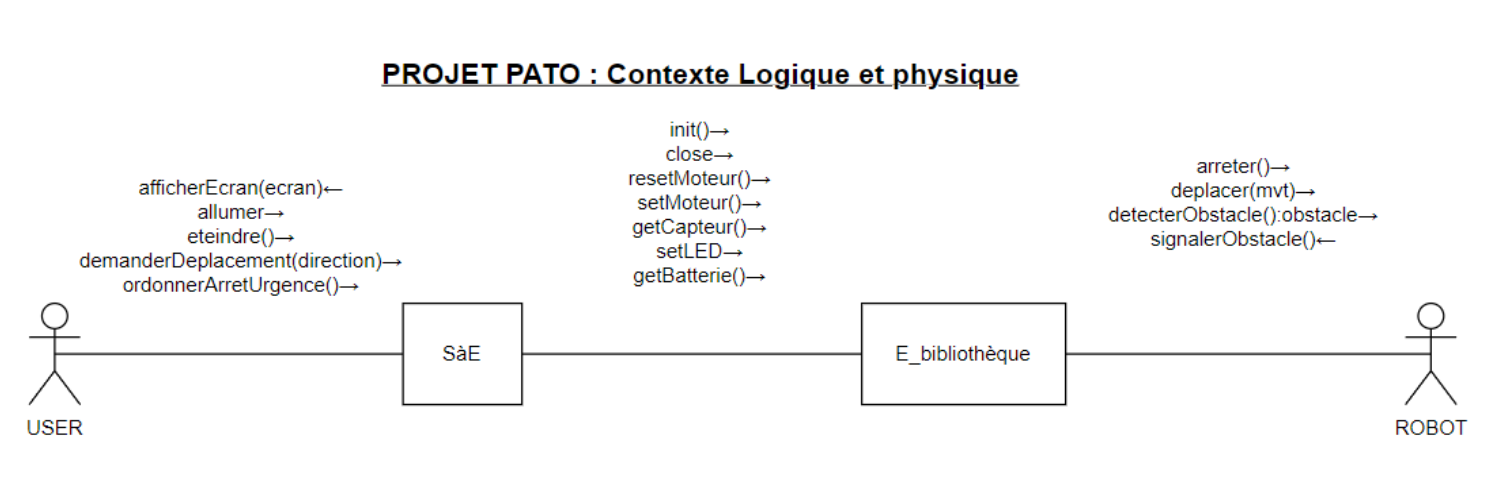
\includegraphics[scale=0.25]{data/contexte_log_phy.png}
    \caption{Contexte logique}
    \label{fig:contexte}
\end{figure}

Le testeur doit pouvoir communiquer avec le SAE via une application Android.

\begin{itemize}
    \item \textbf{afficherEcran(Ecran)} : Grâce à un écran le SAE peut communiquer des informations du robot au testeur
    \item \textbf{allumerRobot()} : Le testeur demande l'allumage du robot via l'application
    \item \textbf{eteindreRobot()} : Le testeur demande l'arrêt du robot via l'application
    \item \textbf{demanderDeplacement(direction)} : Le testeur commande le robot via l'SàE et l'application pour changer la direction du robot
    \item \textbf{ordonnerArretUrgence()} : Le testeur ordonne l'arrêt d'urgence du robot.
\end{itemize}

Le SàE doit pouvoir récupérer les informations via une bibliothèque pour commander le robot.

\begin{itemize}
    \item \textbf{init()} : mrpiz\_init()
    \item \textbf{close()} : mrpiz\_close()
    \item \textbf{setMoteur()} : mrpiz\_motor\_set (mrpiz\_motor\_id id, int cmd)
    \item \textbf{resetMoteur()} : mrpiz\_motor\_encoder\_reset (mrpiz\_motor\_id id)
    \item \textbf{getSensor()} : mrpiz\_proxy\_sensor\_get (mrpiz\_proxy\_sensor\_id id)
    \item \textbf{setLED()} : mrpiz\_led\_rgb\_set (mrpiz\_led\_rgb\_color\_t color)
    \item \textbf{getBatterie()} : cf. fonctions doc batterie
\end{itemize}

La bibliothèque doit envoyer les informations au robot pour pouvoir le faire fonctionner et inversement le robot doit pouvoir renvoyer des informations à la bibliothèque.

\begin{itemize}
    \item \textbf{arreter()} : La bibliothèque peut arrêter le robot
    \item \textbf{déplacer(mvt)} : La bibliothèque fait déplacer le robot
    \item \textbf{detecterObstacle():obstacle} : La bibliothèque donne les informations pour que le robot puisse détecter les obstacles
    \item \textbf{signalerObstacle()} : Le robot renvoie à la bibliothèque les informations sur la signalisation d'obstacle.
\end{itemize}

\subsection{Fonctions principales du système}

Cette section présente les fonctionnalités principales du SàE en utilisant une démarche et une représentation par Cas d'Utilisation (CU).

\subsubsection{Cas d'utilisation}

\CU{
title=              {Evaluer un algorithme},
resume=             {User lance son algorithme dans le logiciel de simulation afin d'y récupérer les métriques associées.},
portee=             {SàE},
niveau=             {Stratégique },
acteursd=           {User, Robot},
acteursi=           {Fournisseur électrique, normes},
preconditions=      {Logiciel lancé et pas en cours d'utilisation, algorithme prêt à être utilisé, connexion au simulateur},
garantiesuccès=     {Consulter les métriques},
garantieminimale=   {Arrêt de la course, Journal de fonctionnement mis à jour},
scenario={
        \begin{minipage}{0.5\textwidth}
            \begin{enumerate}
                \setcounter{enumi}{-1}
                \item User exécute App
                \item App récupère la liste des algos
                \item App récupère l'état du mode « Urgence »
                \item App affiche « Ecran\_Authentification »
                \item User insert ses identifiants de connexion
                \item App affiche « Ecran\_Manuel »
                \item User demande à passer en mode « Nettoyage »
                \item User demande à quitter le mode « Nettoyage »
                \item User quitte App
            \end{enumerate}
        \end{minipage}
    },
variantes={
        \begin{minipage} {0.5\textwidth}
            \begin{enumerate}[label=\arabic*.,ref=\arabic*]
                \setcounter{enumi}{4}
                \item \
                      \begin{enumerate}[label=\theenumi.\alph*.,ref=\theenumi\alph*]
                          \item {[mode « Urgence » désactivé]}
                                \begin{enumerate}[label=\theenumii.\arabic*.,ref=\theenumii\alph*]
                                    \item App affiche Ecran\_Manuel
                                \end{enumerate}
                          \item {[mode « Urgence » activé]}
                                \begin{enumerate}[label=\theenumii.\arabic*.,ref=\theenumii\alph*]
                                    \item App affiche « Ecran\_Urgence »
                                    \item User demande à désactiver le mode « Urgence »
                                    \item Va en 5.a.1.
                                \end{enumerate}
                      \end{enumerate}
                \item \
                      \begin{enumerate}[label=\theenumi.\alph*.,ref=\theenumi\alph*]
                          \item \
                                \begin{enumerate}[label=\theenumii.\arabic*.,ref=\theenumii\alph*]
                                    \item User demande à passer en mode « Nettoyage »
                                \end{enumerate}
                      \end{enumerate}
                \item \
                      \begin{enumerate}[label=\theenumi.\alph*.,ref=\theenumi\alph*]
                          \item \
                                \begin{enumerate}[label=\theenumii.\arabic*.,ref=\theenumii\alph*]
                                    \item User demande à passer en mode « Urgence »
                                \end{enumerate}
                      \end{enumerate}
                \item \
                      \begin{enumerate}[label=\theenumi.\alph*.,ref=\theenumi\alph*]
                          \item \
                                \begin{enumerate}[label=\theenumii.\arabic*.,ref=\theenumii\alph*]
                                    \item User demande à effectuer un déplacement
                                \end{enumerate}
                      \end{enumerate}
                \item \
                      \begin{enumerate}[label=\theenumi.\alph*.,ref=\theenumi\alph*]
                          \item \
                                \begin{enumerate}[label=\theenumii.\arabic*.,ref=\theenumii\alph*]
                                    \item User demande à quitter le mode « Nettoyage »
                                \end{enumerate}
                      \end{enumerate}
                \item \
                      \begin{enumerate}[label=\theenumi.\alph*.,ref=\theenumi\alph*]
                          \item \
                                \begin{enumerate}[label=\theenumii.\arabic*.,ref=\theenumii\alph*]
                                    \item User demande à passer en mode « Urgence »
                                \end{enumerate}
                      \end{enumerate}

            \end{enumerate}
        \end{minipage}
    },
extensions={
    \begin{minipage}{0.5\textwidth}
        \begin{enumerate} [label=*.,ref=*]
            \item  {[Perte de connexion côté Simu]}
            \begin{enumerate} [label=\theenumi.\arabic*.,ref=\theenumi\alph*]
                \item App affiche « Ecran\_Perte\_Connexion »
                \end{enumerate}
        \end{enumerate}
        
    \end{minipage}
},
infos={}
}

\subsubsection{Diagramme de classe}

\begin{figure}[H]
    \center
    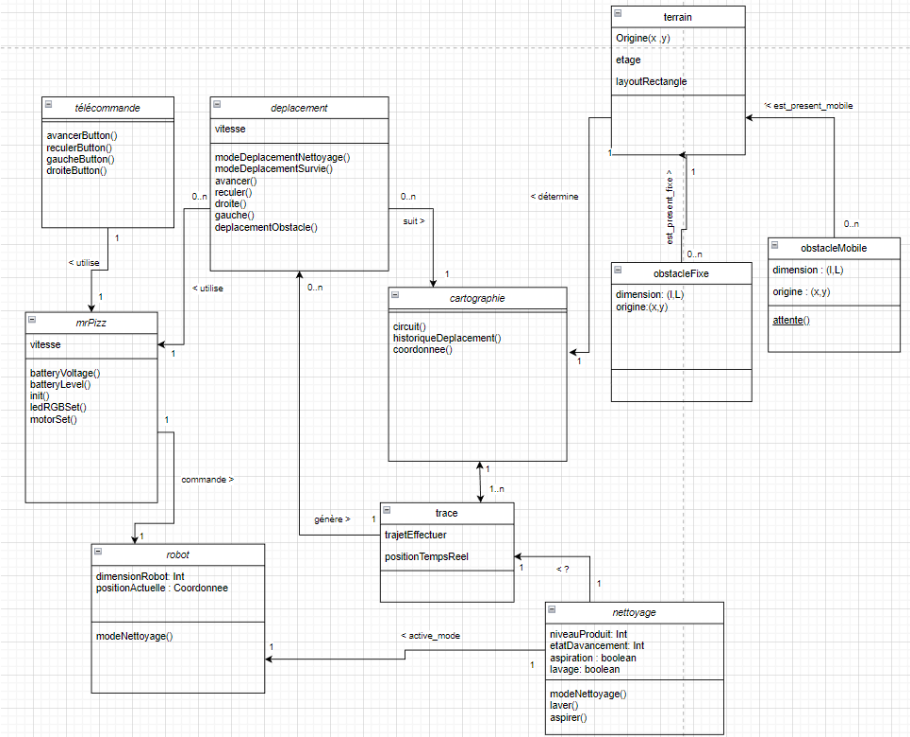
\includegraphics[scale=0.5]{data/diag_class.png}
    \caption{Diagramme de classe}
    \label{fig:diagramme_classe}
\end{figure}

\subsubsection{Diagramme de séquence}